\documentclass{standalone}
%-----------------------------------------------------------------------------%
%%% Math %%%
\usepackage{amsmath,mathtools,amssymb,mathrsfs}
% \usepackage{centernot}
% \usepackage{accents}
% \usepackage[makeroom]{cancel}
% \newcommand{\raum}{\phantom{=}{\:\,}}
% \newcommand{\asDemonstrated}{\null\nobreak\hfill\ensuremath{\blacksquare}}
%-----------------------------------------------------------------------------%
%%% Color %%%
\usepackage[dvipsnames]{xcolor}
\definecolor{myred}{RGB}{229,0,0}
\definecolor{myblue}{RGB}{0,98,144}
\definecolor{myyellow}{RGB}{246,182,50} % {225,217,0} colorblind
\definecolor{mygrey}{RGB}{120,120,120} % {225,217,0} colorblind
\newcommand{\red}[1]{\textcolor{myred}{#1}}
\newcommand{\grey}[1]{\textcolor{mygrey}{#1}}
\newcommand{\blue}[1]{\textcolor{myblue}{#1}}
\newcommand{\yellow}[1]{\textcolor{myyellow}{#1}}
%-----------------------------------------------------------------------------%
%%% TikZ %%%
\usepackage{tikz}
\usetikzlibrary{calc}
% \usetikzlibrary{positioning}
% \usetikzlibrary{patterns}
% \usetikzlibrary{fit}
% \usetikzlibrary{angles,quotes}
% \usetikzlibrary{intersections}
% \usetikzlibrary{decorations.markings}
%-----------------------------------------------------------------------------%

\begin{document}

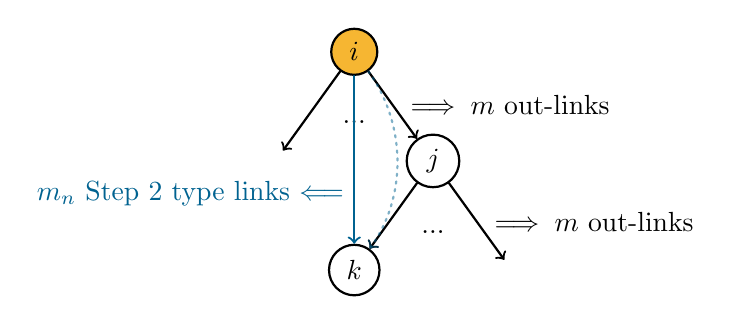
\begin{tikzpicture}[thick,line cap=round,scale=2,yscale=0.8]
	\tikzstyle{bai}=[solid,circle,draw,fill=white,inner sep=.8pt];
	\tikzstyle{hei}=[solid,circle,draw,fill=black,inner sep=.8pt];
	\node[circle,draw,fill=myyellow] (i)  at (0,0)           {$i$};
	\node[circle,draw] (j)  at (-60:1)         {$j$};
	\node              (j') at (240:1)         {};
	\node              (jm) at (-90:1)         {};
	\node              (k') at ($(j)+(-60:1)$) {};
	\node[circle,draw] (k)  at ($(j)+(240:1)$) {$k$};
	\node              (km) at ($(j)+(-90:1)$) {};
	\draw[->] (i) -- node[right]{$\implies m$ out-links} (j);
	\draw[->] (i) -- (j');
	\draw[->] (j) -- (k);
	\draw[->] (j) -- node[right]{$\implies m$ out-links} (k');
	\path (i) -- node[pos=0.5]{$...$} (jm);
	\path (j) -- node[pos=0.5]{$...$} (km);
	\draw[->,myblue] (i) -- node[pos=0.7,left]{$m_{n}$ Step 2 type links $\Longleftarrow$} (k);
	\draw[->,myblue,dotted,opacity=0.5] (i) .. controls ($(i)!2/3!(j)$) and ($(j)!1/3!(k)$) .. (k);
\end{tikzpicture}

\end{document}
